\documentclass[11pt]{article}

\usepackage{amsmath,amsfonts,amssymb}
\usepackage{graphicx}
\usepackage{hyperref}
\usepackage{geometry}
\usepackage{booktabs}
\geometry{margin=1in}

\title{Structural Admissibility:\\
An I2OS Framework for Secure Generative Systems}

\author{Anonymous}

\date{2026}

\begin{document}

\maketitle

\begin{abstract}
We introduce Structural Admissibility, a security framework for generative systems based on transition validity rather than post-generation filtering. Unlike conventional AI safety mechanisms that filter outputs after generation, the proposed I2OS framework permits execution only when a state transition is structurally admissible. The framework integrates admissibility constraints, reality confirmation, and collapse detection. This redefines safety as a non-collapse constraint over state transitions. We further present a use case for LLM hallucination suppression by reformulating hallucination as an unsupported state transition. The approach is domain-independent and applicable to generative AI, financial systems, discourse analysis, and autonomous systems.
\end{abstract}

\section{Introduction}

Modern AI systems rely on optimization, prediction, and post-hoc filtering for safety. However, these approaches allow unsafe intermediate states.

Conventional pipeline:
\[
Generate \rightarrow Filter
\]

Proposed:
\[
Allow\ execution\ only\ if\ admissible
\]

\textbf{Core Claim:}
\begin{quote}
A system is safe if and only if it executes only structurally admissible transitions.
\end{quote}

\section{Structural Admissibility}

\subsection{Definition}

A transition is structurally admissible when the current state, transition operator, and resulting state satisfy a structural constraint:

\[
C(S_t, T, S_{t+1}) = 1
\]

where $S_t$ is the current state, $T$ is the candidate transition, $S_{t+1}$ is the resulting state, and $C$ is the admissibility constraint.

\subsection{Execution Rule}

\[
GO =
\mathbf{1}
[
C(S_t, T, S_{t+1}) = 1
]
\]

Execution occurs only when the transition is admissible.

\section{I2OS Security Model}

\subsection{Core Equation}

\[
GO(t) =
\mathbf{1}
[
\Gamma(Q(t')) R(t') > \theta
\land Reality(t)=1
\land \neg Collapse(t)
]
\]

\subsection{Components}

Question generation:
\[
Q = |\nabla M|
\]

Resonance:
\[
R = \Phi \cdot \eta_{sync} \cdot (1 - \Delta \phi)
\]

Structure generation:
\[
S_{new} = \Gamma(Q)
\]

Reality confirmation:
\[
Reality(t) =
\mathbf{1}[\Delta p_{fav} > \theta]
\]

Collapse detection:
\[
Collapse(t) =
\mathbf{1}[\min(F,\Sigma,E) < \theta_c]
\]

\textbf{Security Principle:}
\[
Security = NonCollapseConstraint
\]

\section{Architecture}

\begin{figure}[h]
\centering
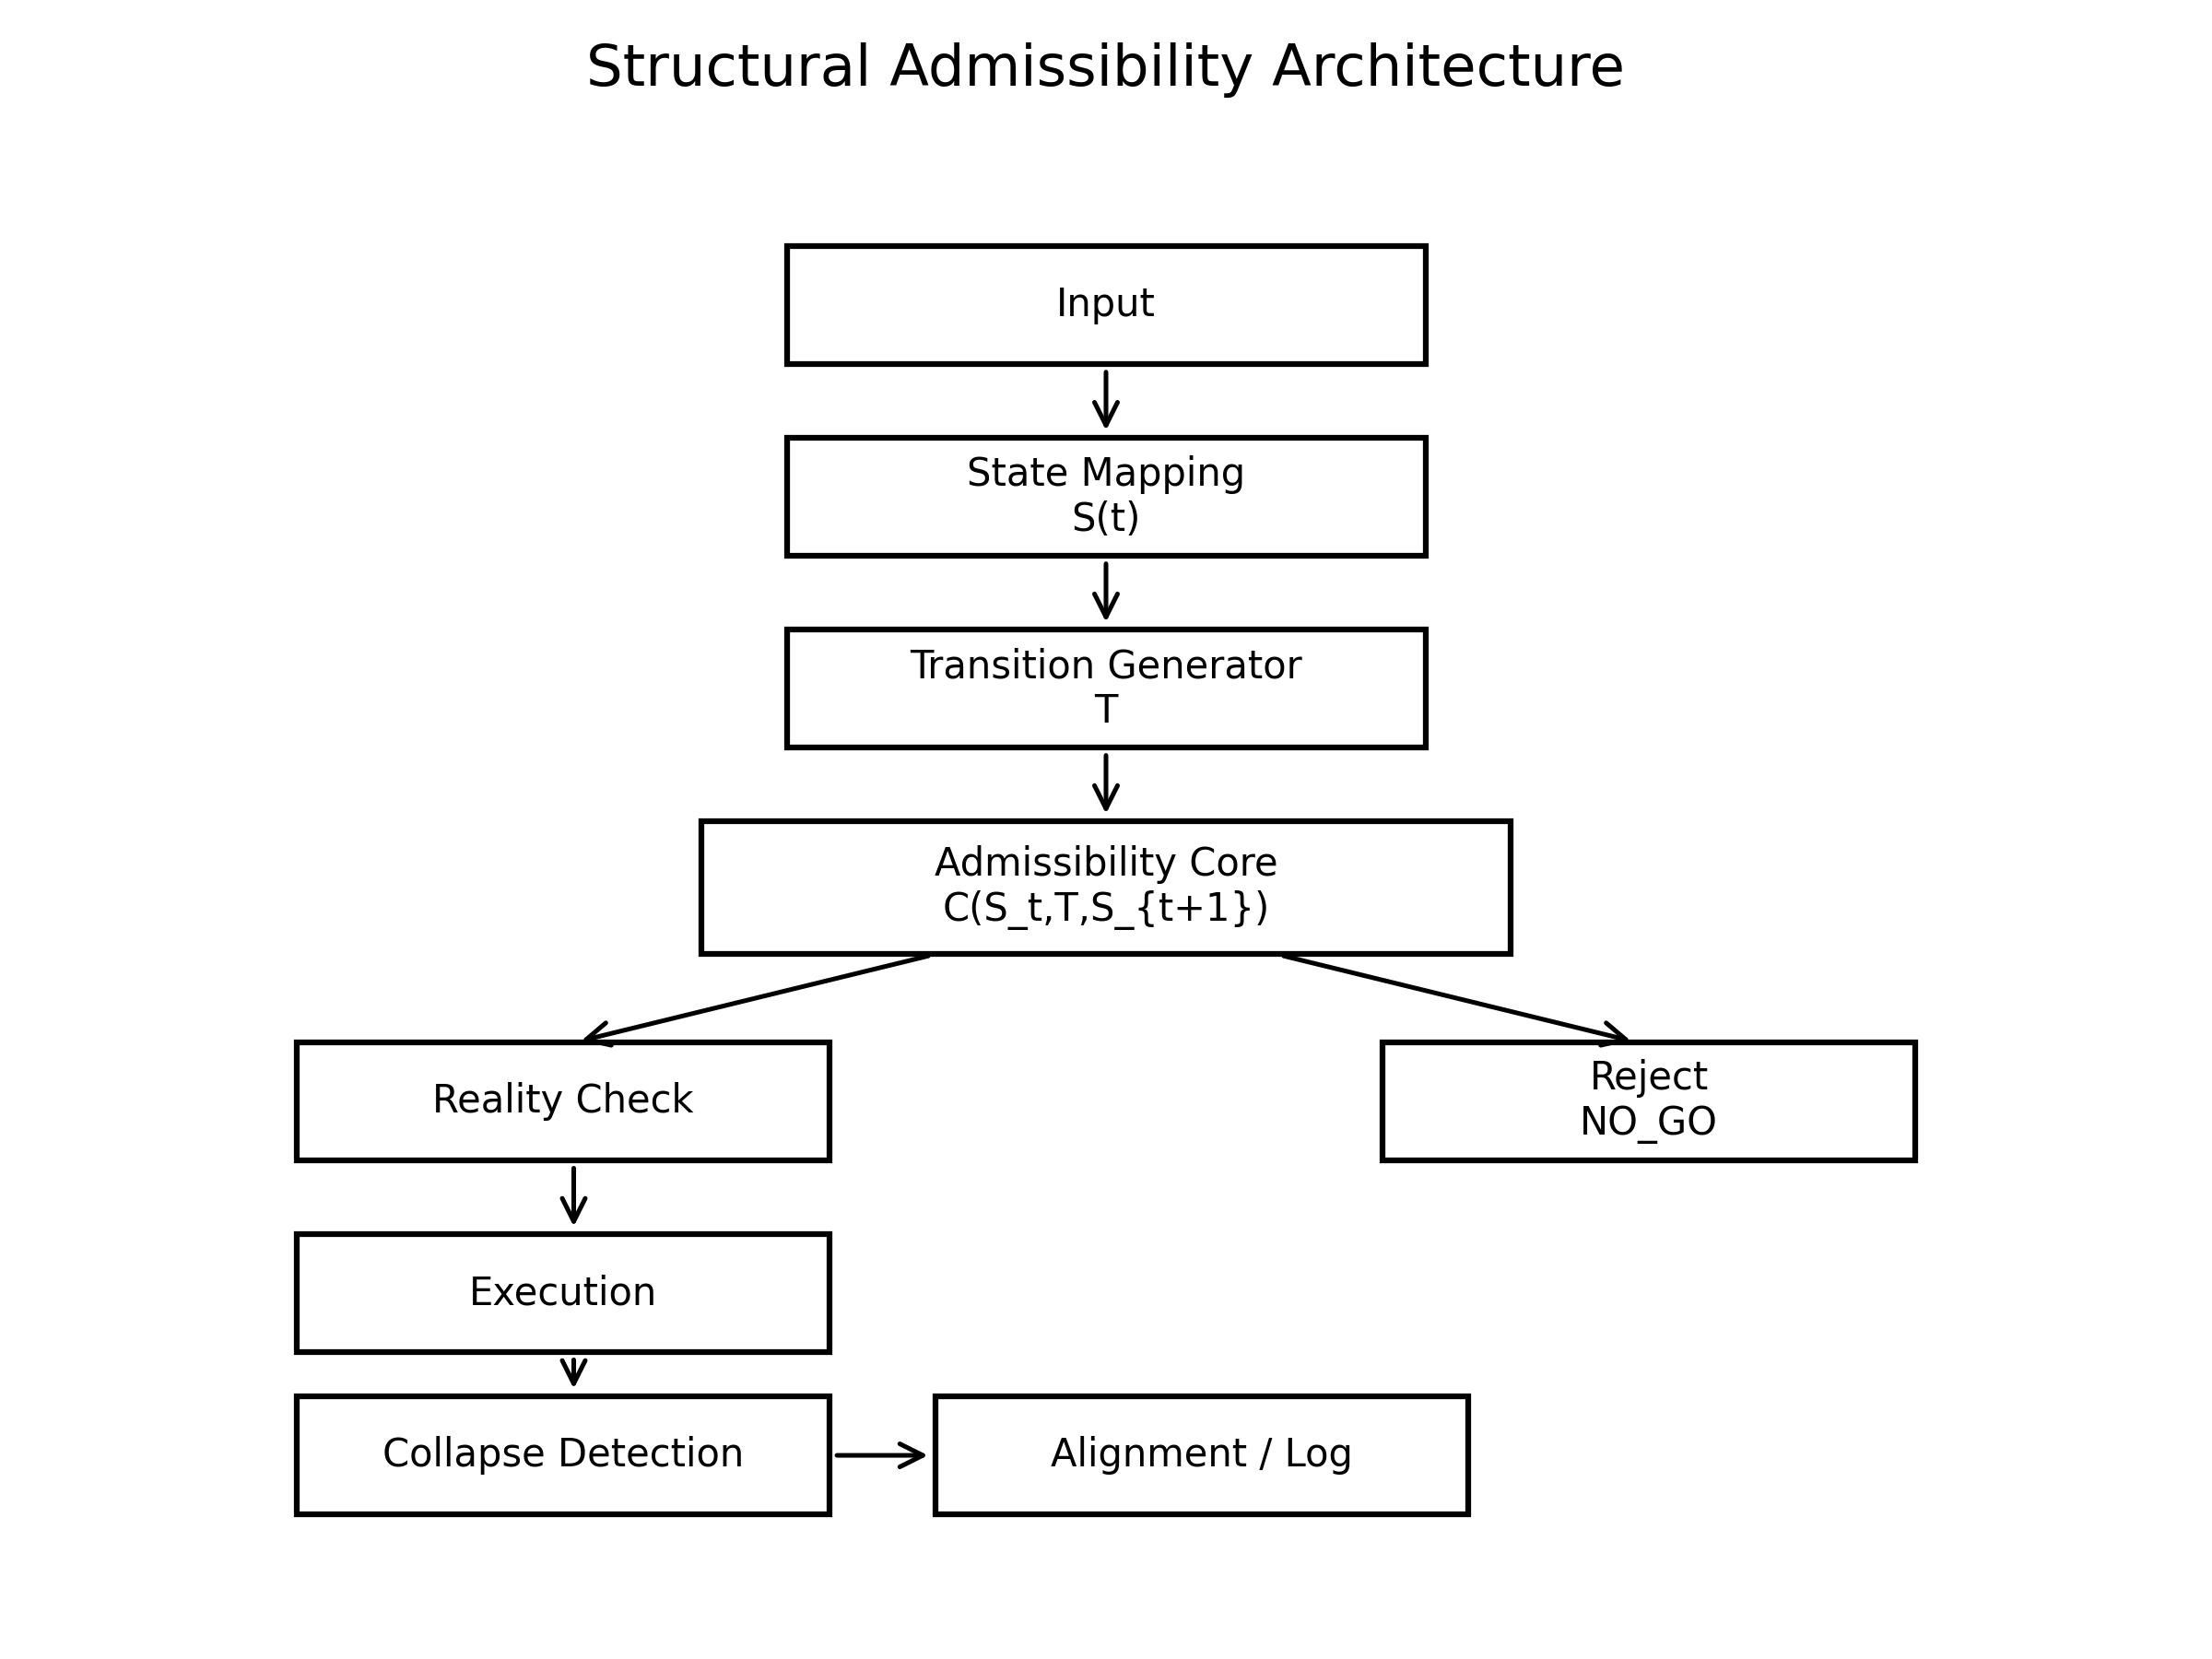
\includegraphics[width=0.9\linewidth]{../figures/fig1_architecture.png}
\caption{Structural Admissibility Architecture.}
\end{figure}

\section{Comparison with Conventional Safety}

\begin{figure}[h]
\centering
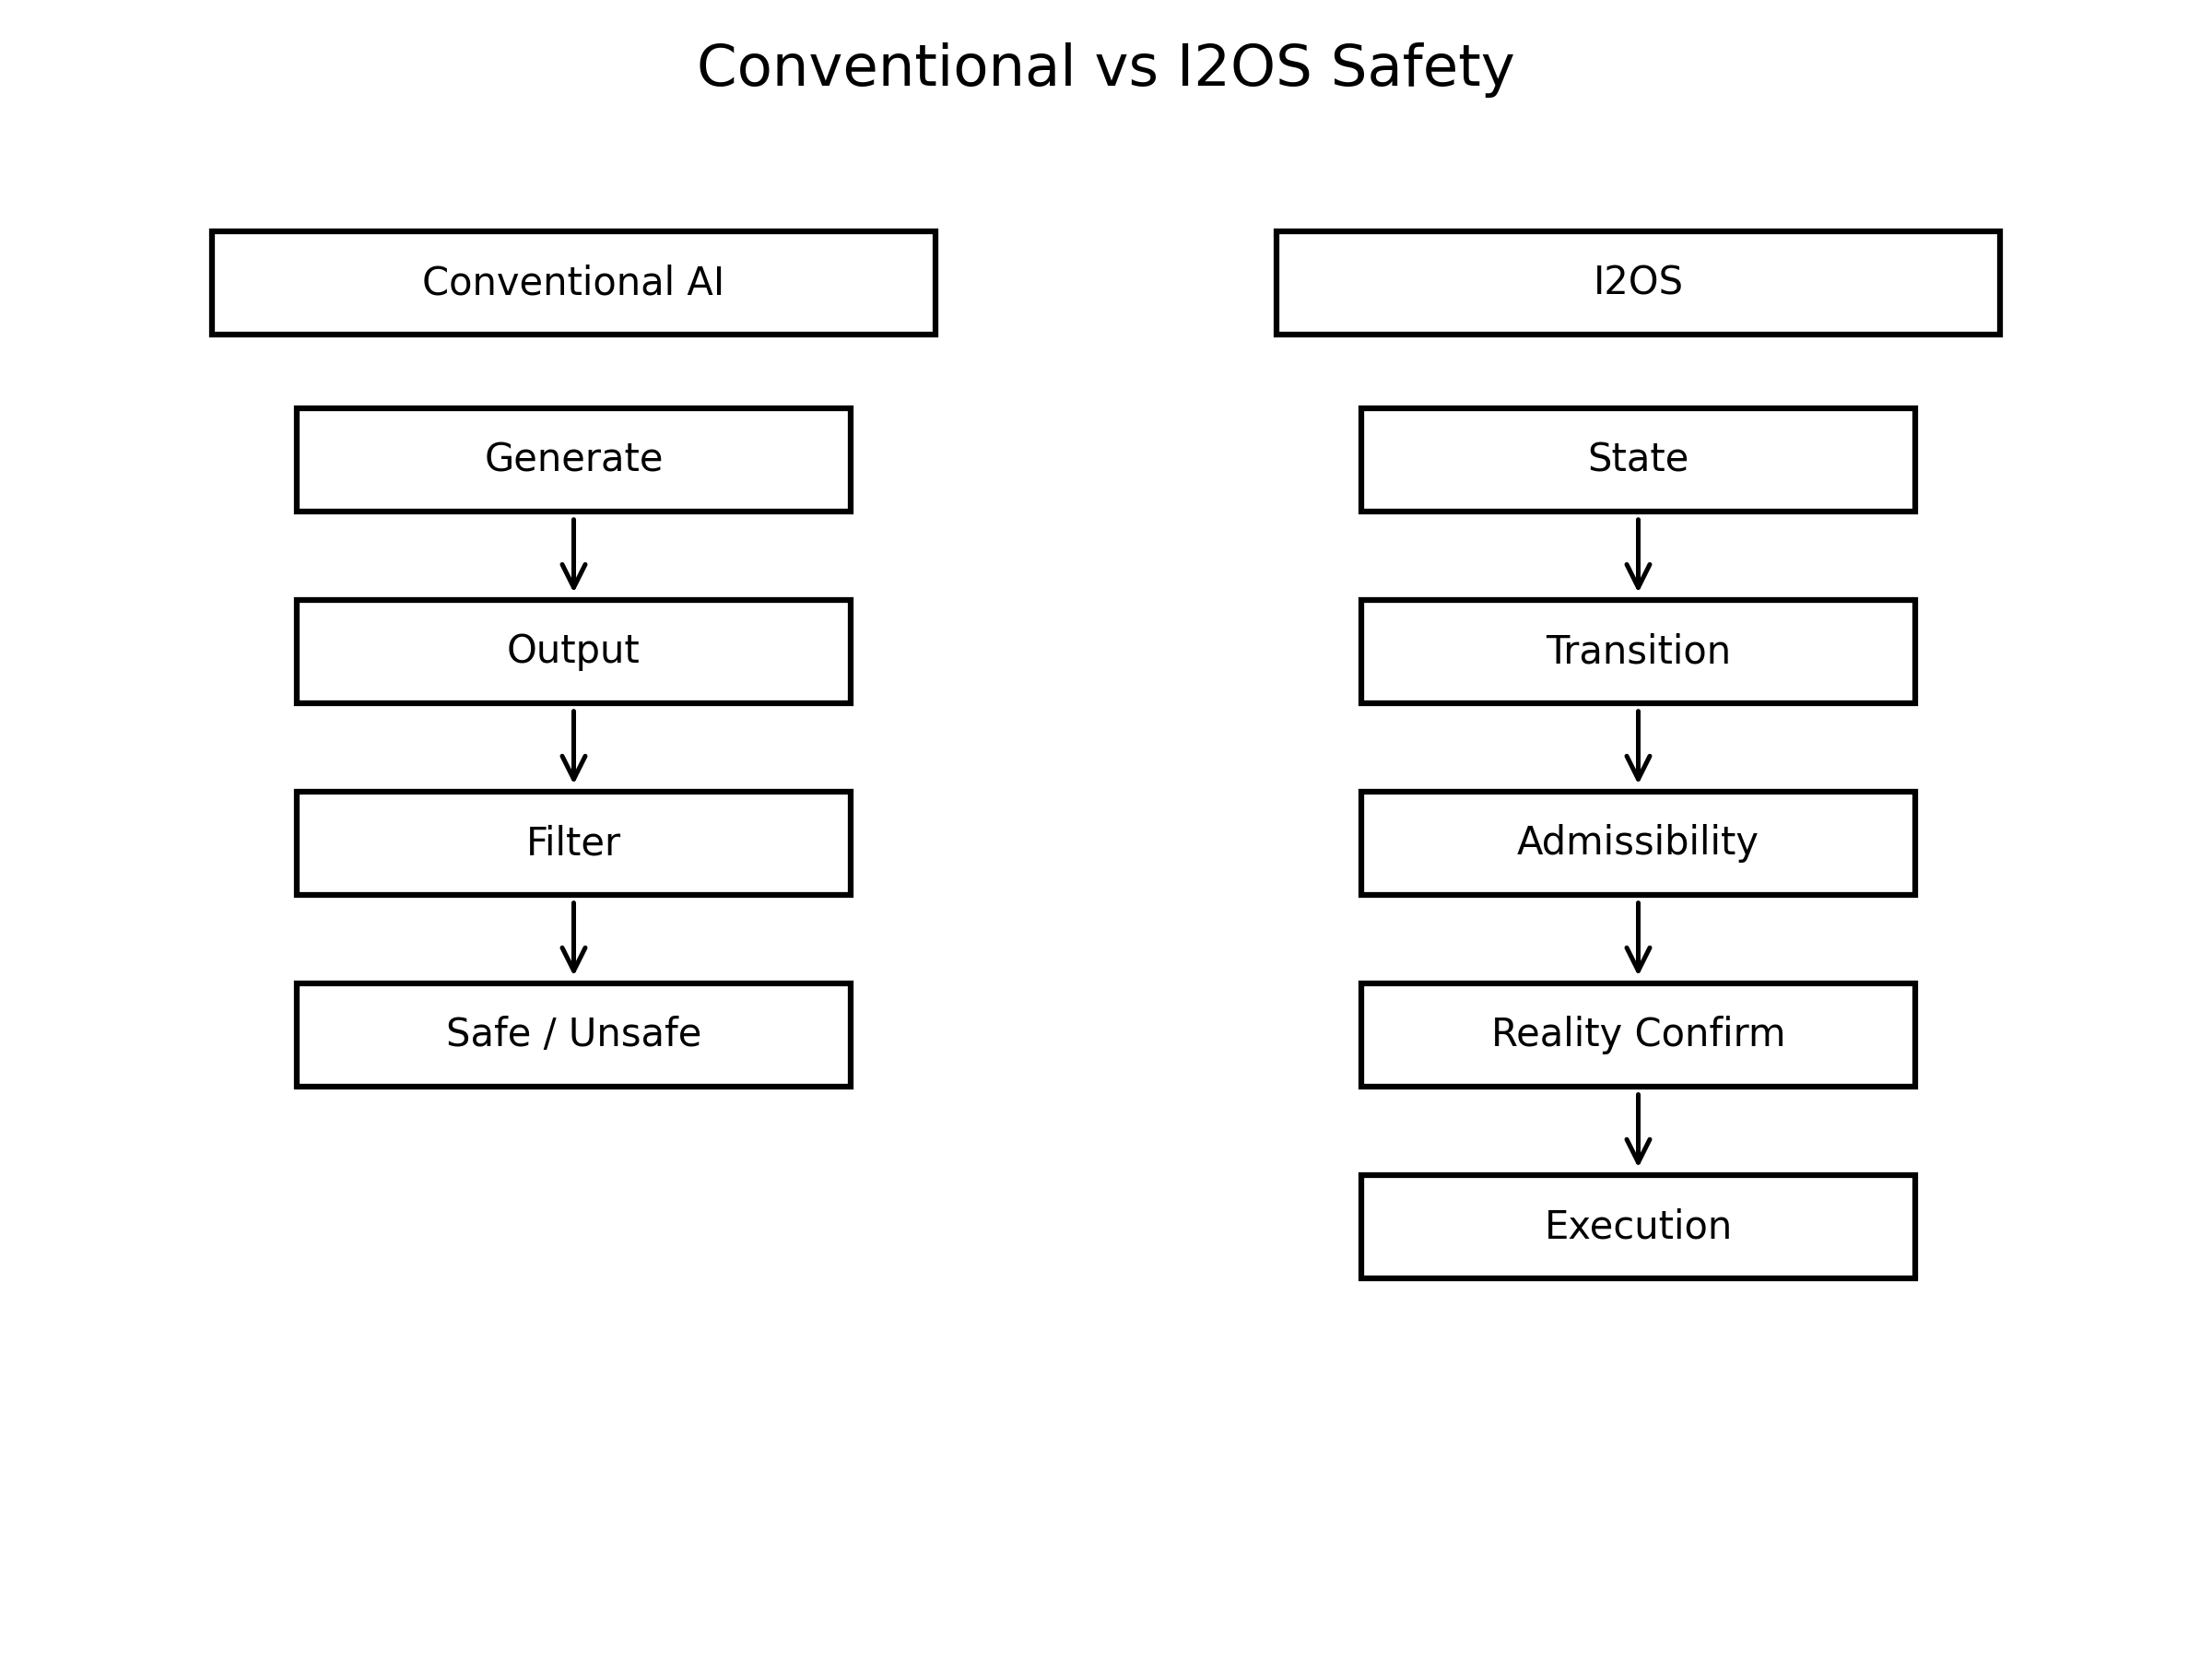
\includegraphics[width=0.9\linewidth]{../figures/fig2_comparison.png}
\caption{Conventional vs I2OS Safety.}
\end{figure}

\section{Admissibility Funnel}

\begin{figure}[h]
\centering
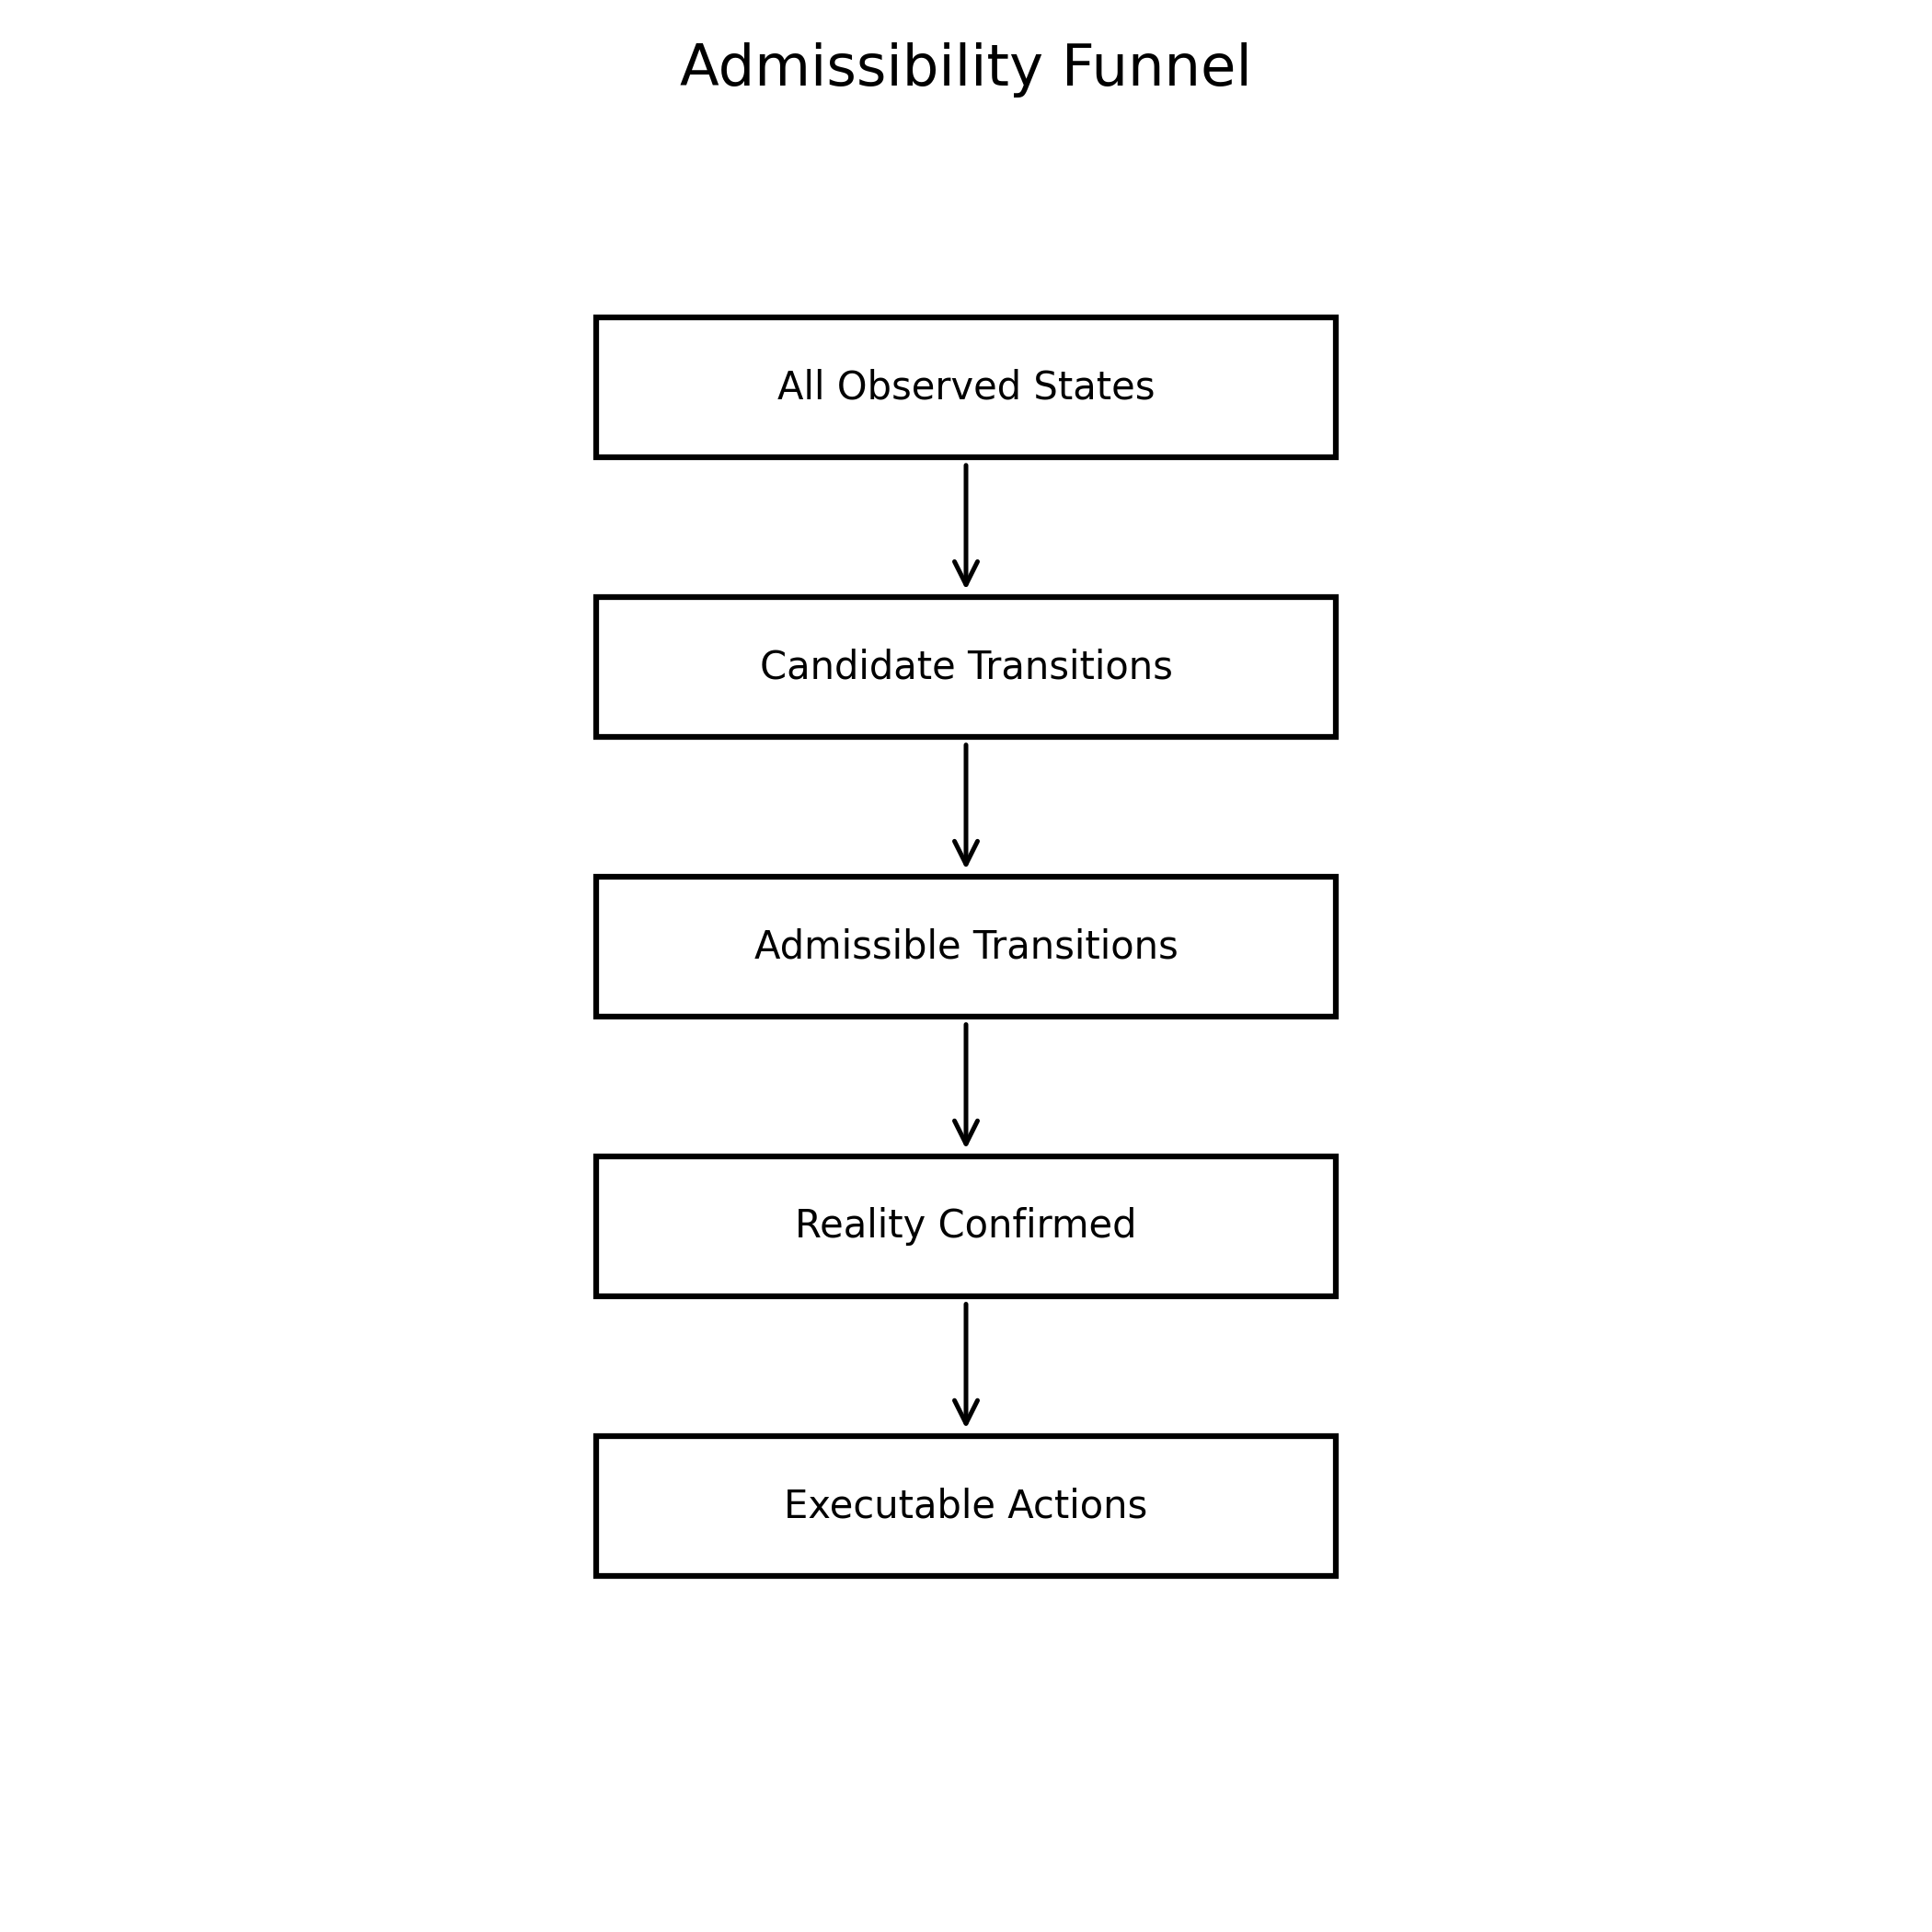
\includegraphics[width=0.9\linewidth]{../figures/fig3_funnel.png}
\caption{Admissibility Funnel.}
\end{figure}

\section{Admissible Region}

\begin{figure}[h]
\centering
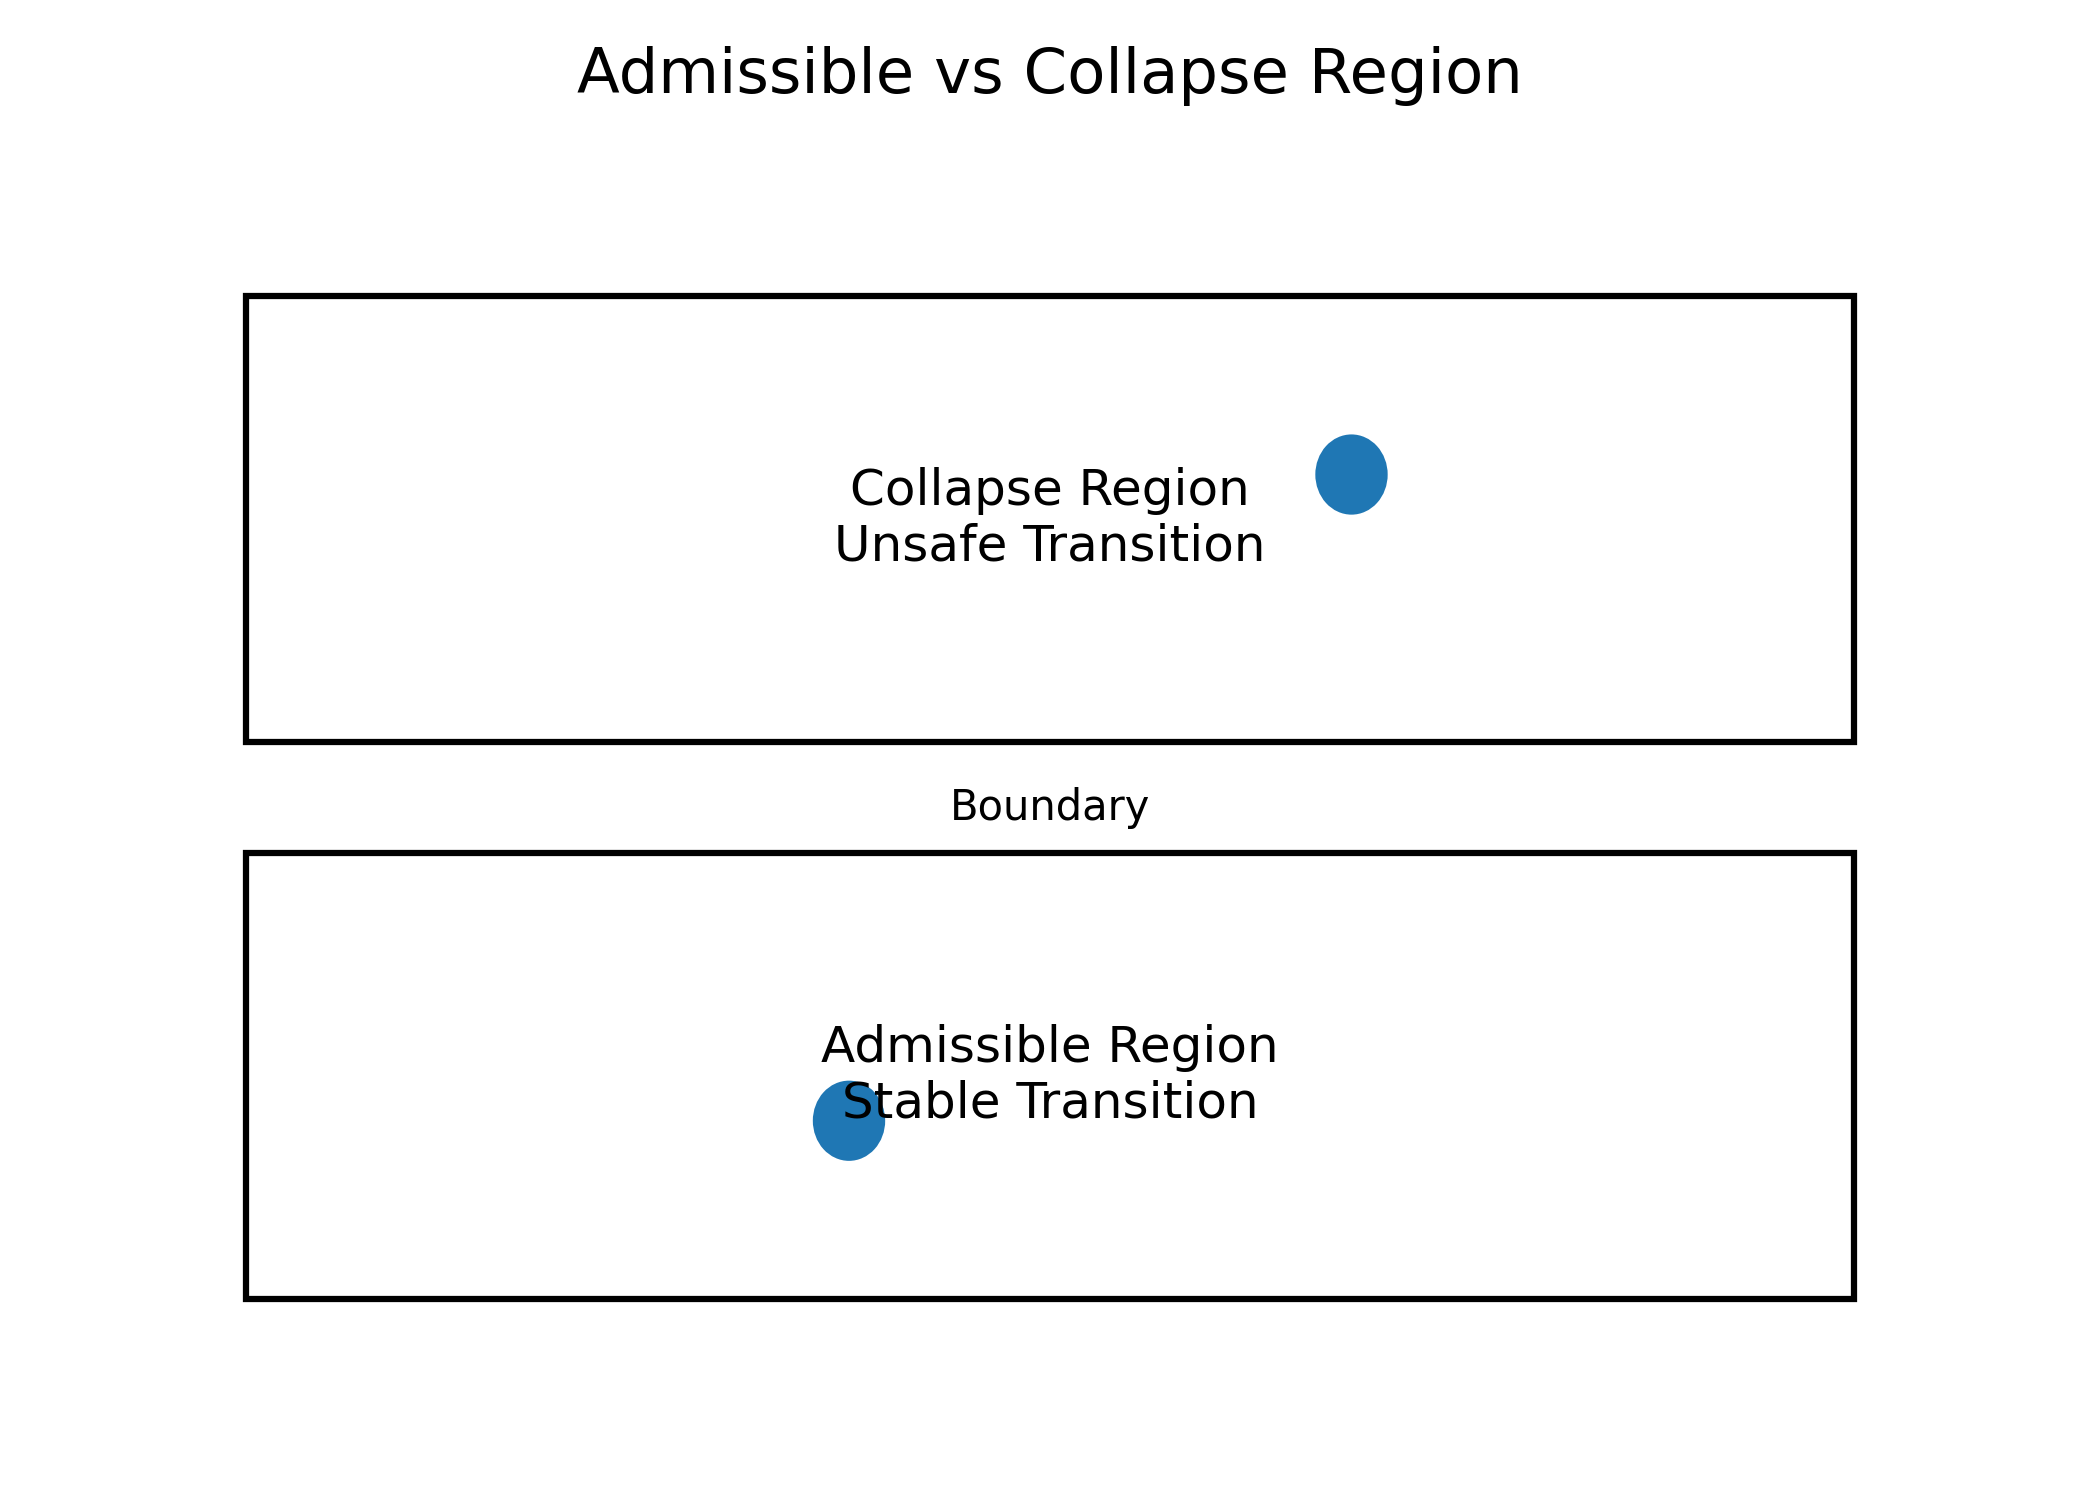
\includegraphics[width=0.9\linewidth]{../figures/fig4_region.png}
\caption{Admissible vs Collapse Region.}
\end{figure}

\section{Experimental Evaluation}

\subsection{Objective}

The objective is to validate that execution should occur only under admissible transitions with real-world confirmation.

\subsection{Setup}

\[
S(t) = (F, \Sigma, E, \phi, P, E_{res}, Pr)
\]

Baseline:
\[
GO_{baseline} = \mathbf{1}[Pr > \theta]
\]

Proposed:
\[
GO_{proposed} =
\mathbf{1}[C \land V \land R \land \neg Collapse]
\]

\subsection{Results}

Baseline:
\begin{itemize}
\item Many entries
\item Late execution
\item Weak favorable movement
\end{itemize}

Proposed:
\begin{itemize}
\item Fewer entries
\item Strong filtering
\item Higher quality execution
\end{itemize}

\subsection{Key Insight}

\begin{quote}
Execution $\neq$ Structural Alignment
\end{quote}

\[
Execution = Admissible\ Transition
\]

\begin{figure}[h]
\centering
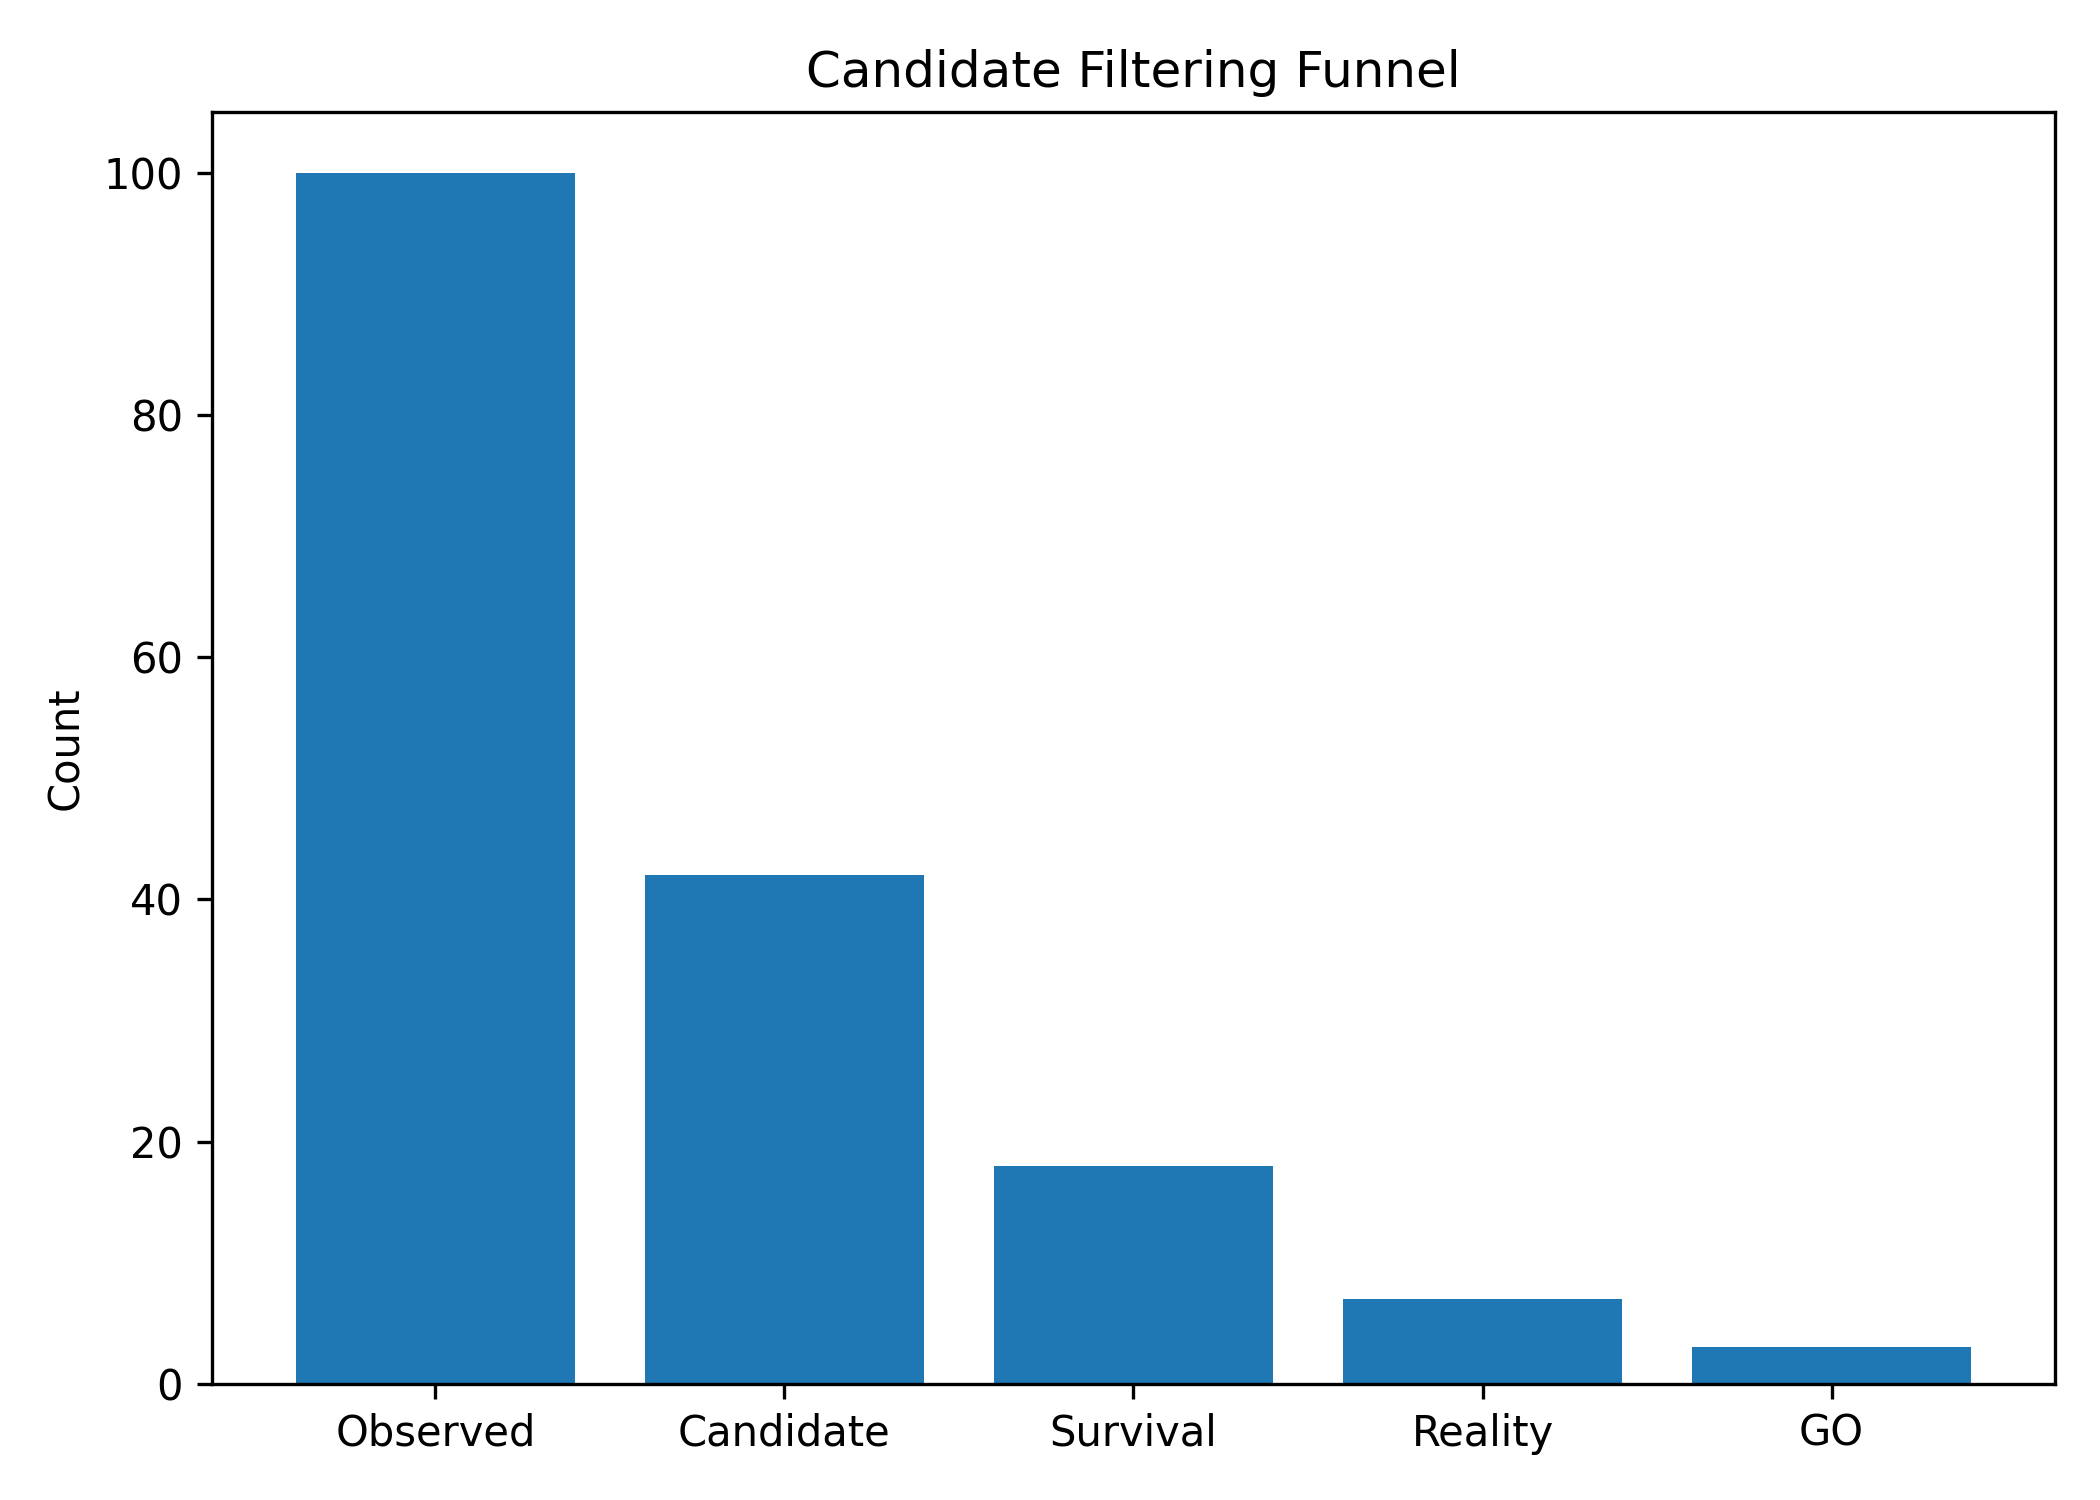
\includegraphics[width=0.9\linewidth]{../figures/fig5_candidate_funnel.png}
\caption{Candidate Filtering Funnel.}
\end{figure}

\begin{figure}[h]
\centering
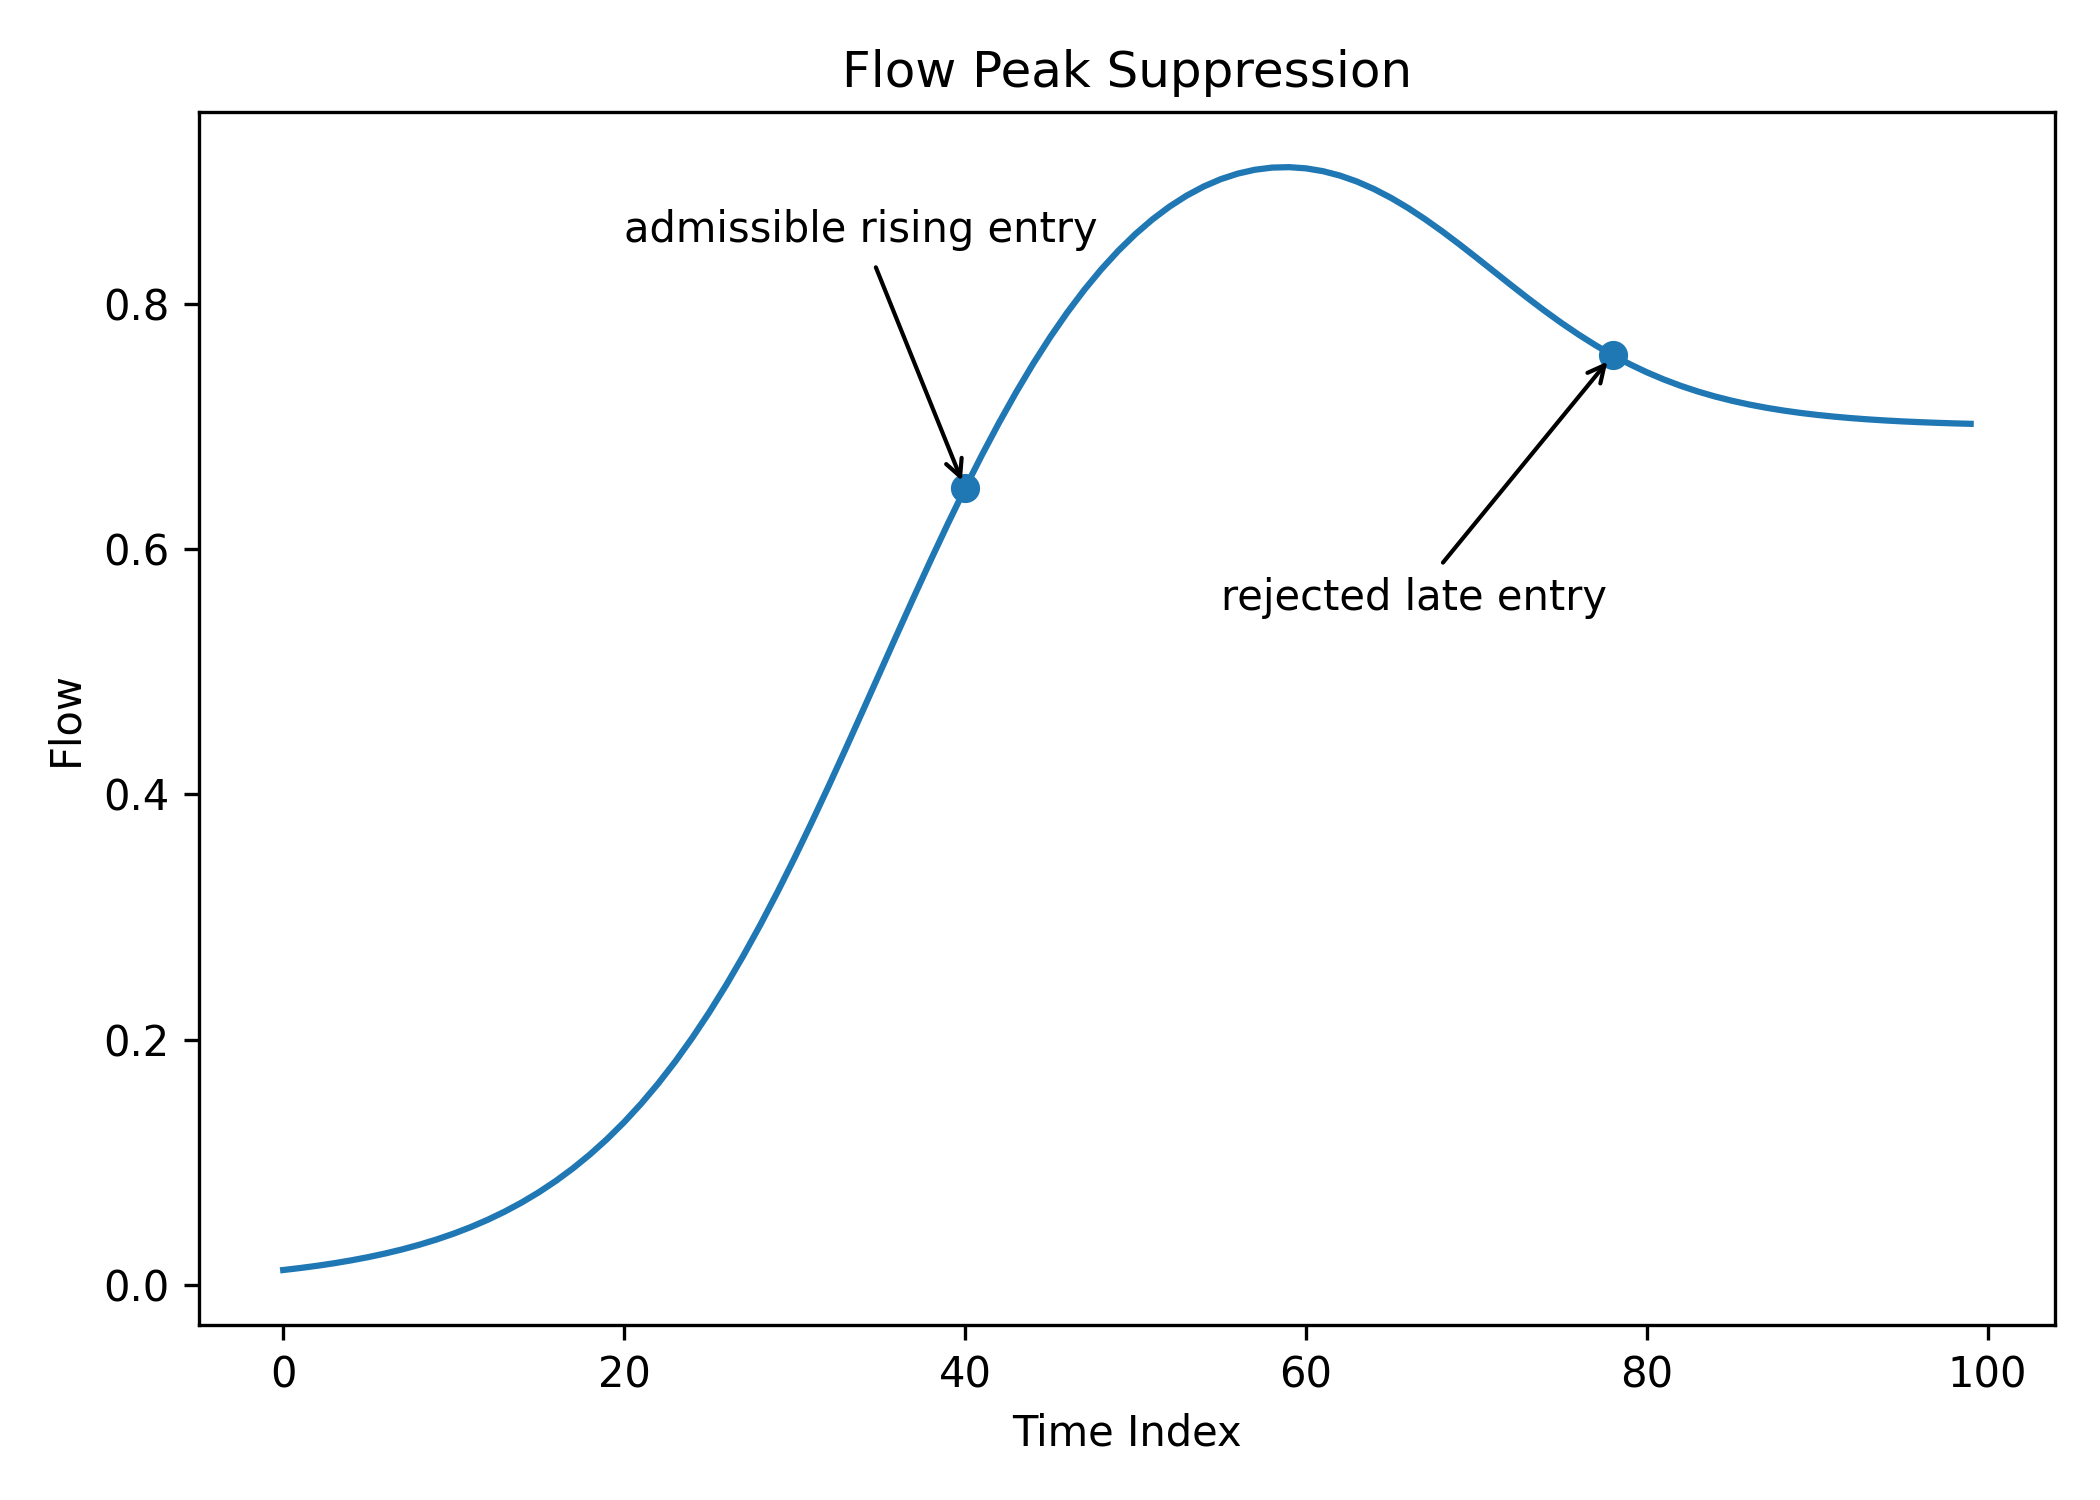
\includegraphics[width=0.9\linewidth]{../figures/fig6_flow_dynamics.png}
\caption{Flow Peak Suppression.}
\end{figure}

\begin{table}[h]
\centering
\caption{Baseline vs Proposed Execution Models.}
\begin{tabular}{lccccc}
\toprule
Method & Entries & MFE & MAE & Fail Rate & Positive \\
\midrule
Baseline & -- & -- & -- & -- & -- \\
Proposed & -- & -- & -- & -- & -- \\
\bottomrule
\end{tabular}
\end{table}

\section{Use Case: LLM Hallucination Suppression}

\subsection{Problem Definition}

Large Language Models are known to produce hallucinated outputs, i.e., statements that are not supported by evidence or context.

Conventional approaches treat hallucination as an output-level problem:

\[
Generate \rightarrow Verify \rightarrow Filter
\]

This approach is reactive and allows unsupported intermediate states.

\subsection{Structural Reformulation}

We redefine hallucination as a structural phenomenon:

\begin{quote}
Hallucination is an unsupported state transition from context to output.
\end{quote}

Let:

\begin{itemize}
\item $S_t$: current conversational context
\item $T$: candidate generation transition
\item $S_{t+1}$: generated output state
\end{itemize}

\subsection{Admissibility Condition for LLMs}

\[
GO_{LLM} =
\mathbf{1}
[
C(S_t,T,S_{t+1}) = 1
\land G(S_{t+1}) = 1
\land \neg H(S_{t+1})
]
\]

where $C$ denotes structural admissibility, $G$ denotes grounding condition, and $H$ denotes hallucination risk.

\subsection{Decomposition of Constraints}

\[
C_{LLM} =
\mathbf{1}
[
C_{ctx}
\land C_{src}
\land C_{cause}
\land C_{scope}
\land C_{uncert}
]
\]

\begin{itemize}
\item $C_{ctx}$: Context consistency
\item $C_{src}$: Source grounding
\item $C_{cause}$: Causal continuity
\item $C_{scope}$: Scope boundedness
\item $C_{uncert}$: Uncertainty preservation
\end{itemize}

\subsection{Execution Modes}

\begin{itemize}
\item Admissible $\rightarrow$ Full response
\item Partially admissible $\rightarrow$ Qualified response
\item Non-admissible $\rightarrow$ Refusal or clarification request
\end{itemize}

\begin{figure}[h]
\centering
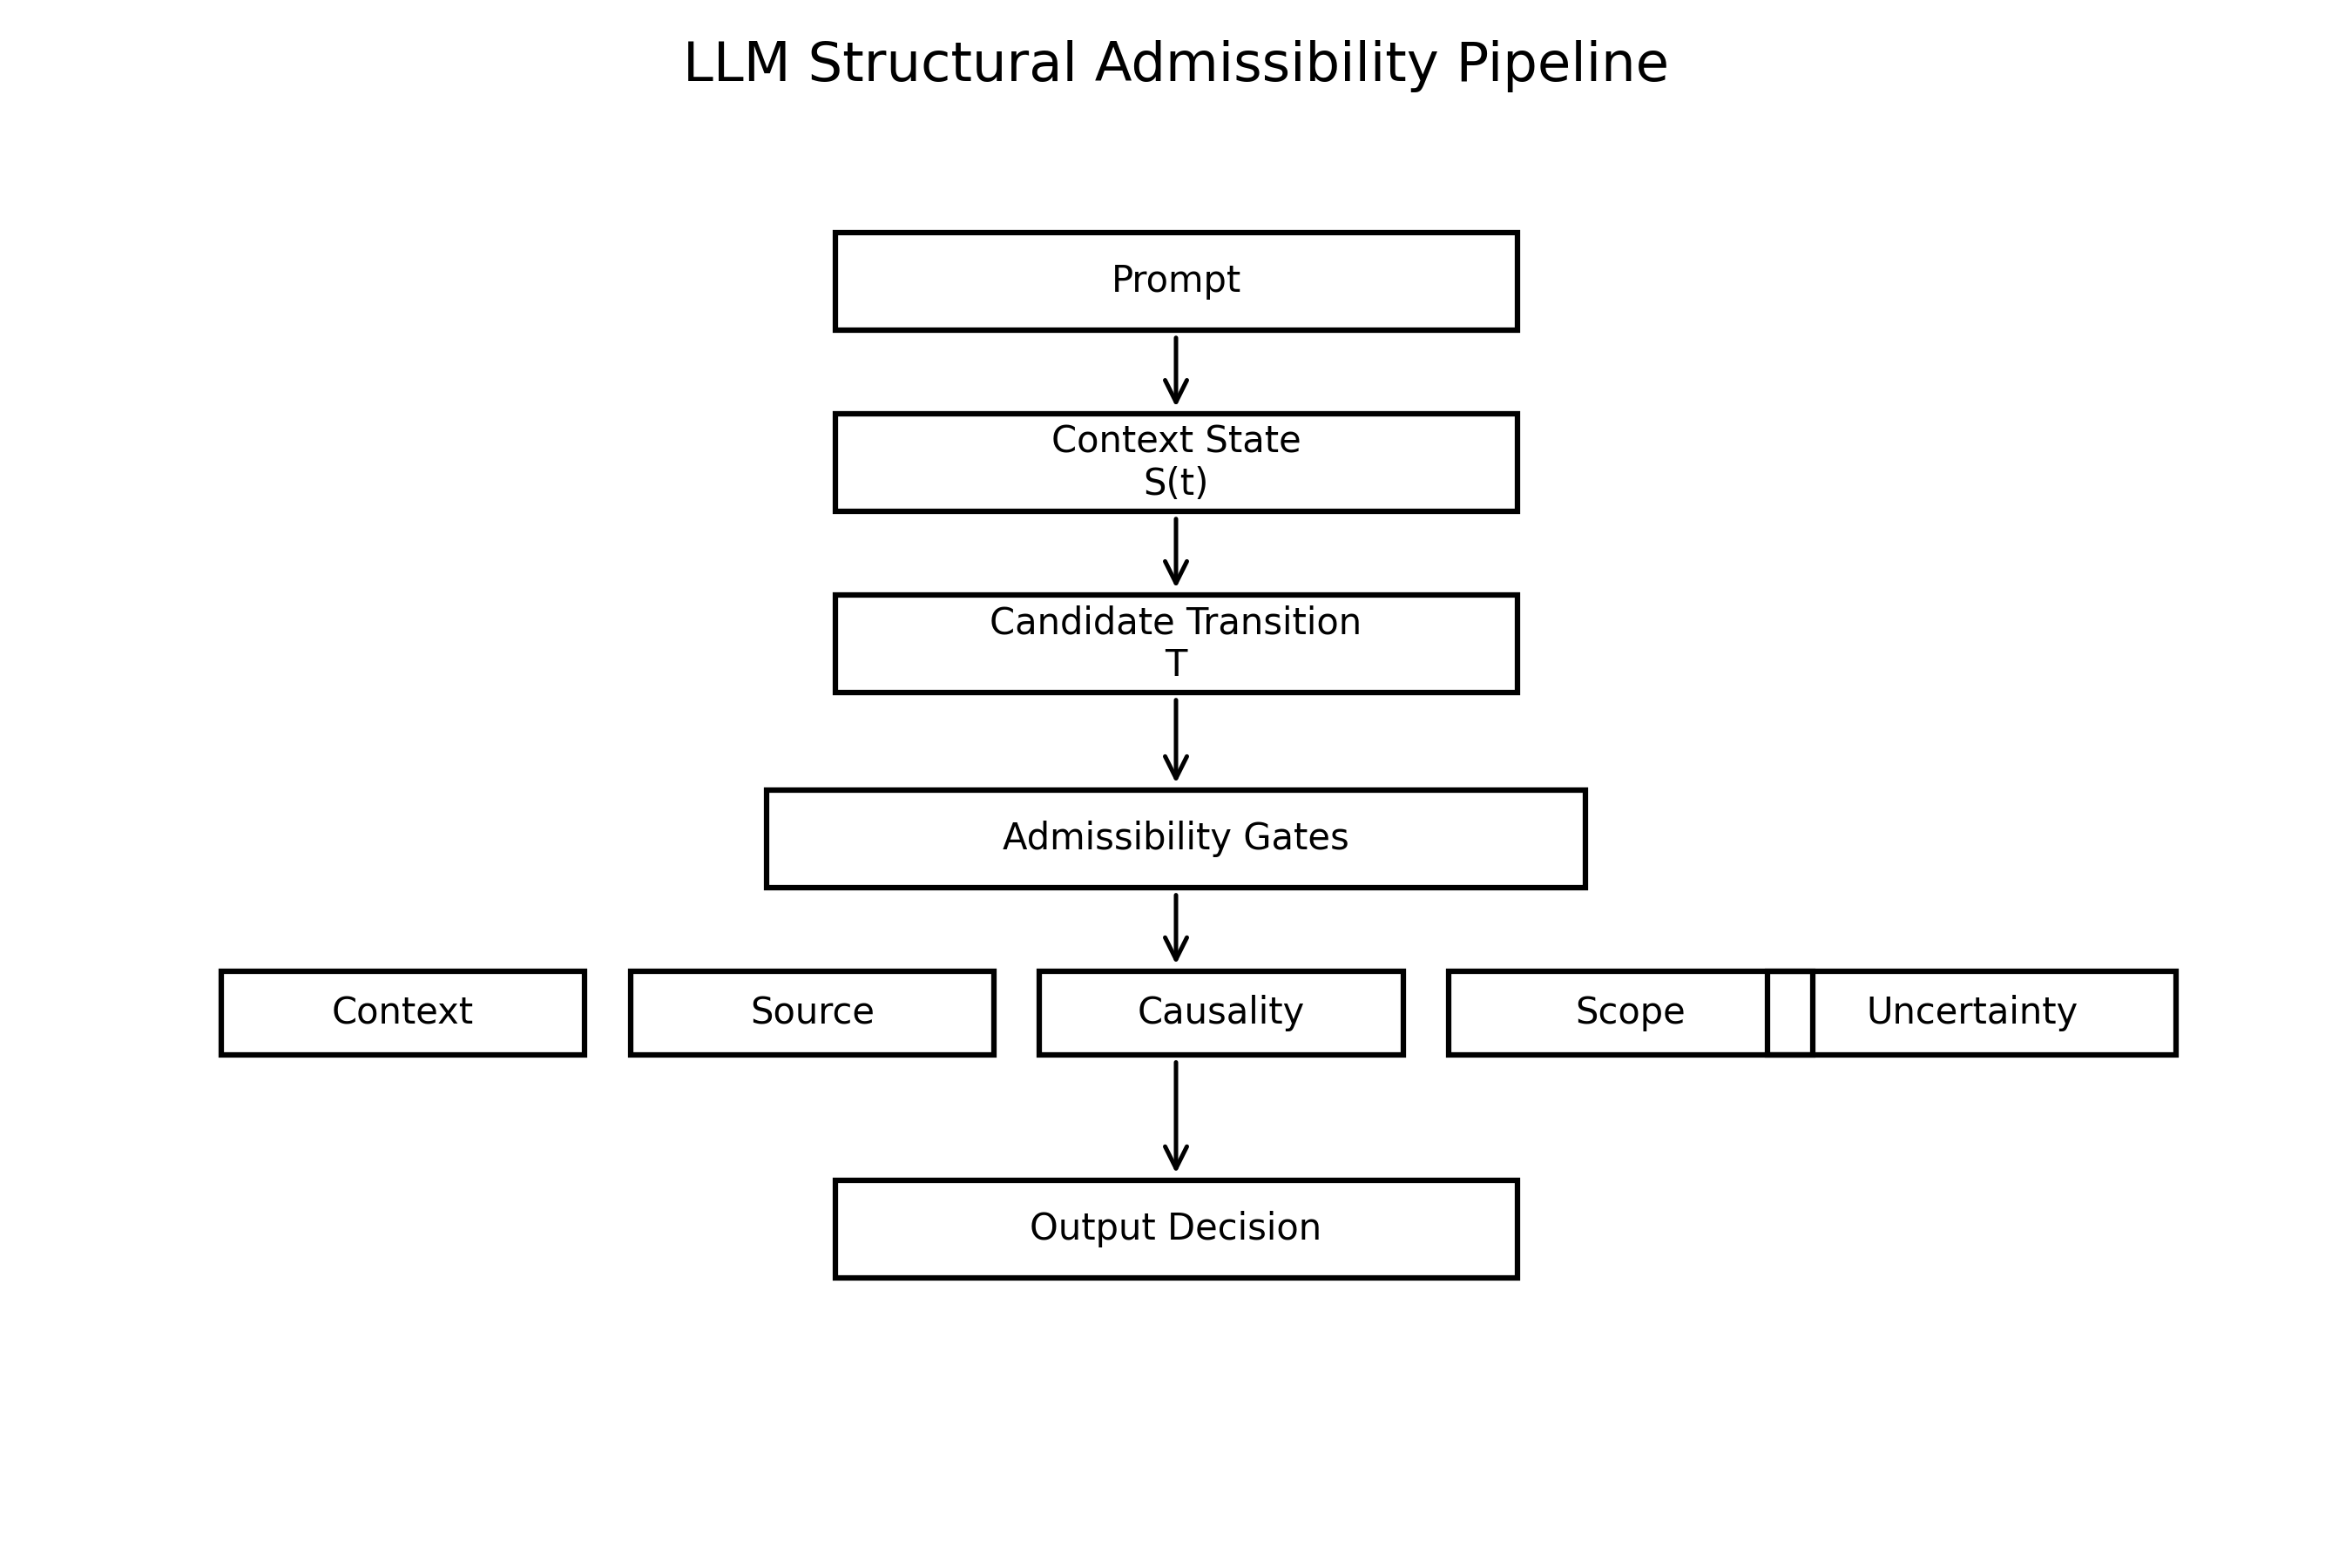
\includegraphics[width=0.9\linewidth]{../figures/fig9_llm_admissibility.png}
\caption{LLM Structural Admissibility Pipeline.}
\end{figure}

\subsection{LLM Hallucination Experiment}

We evaluate the proposed framework on three representative prompt types:

\begin{itemize}
\item Fact-based prompts with incomplete knowledge
\item Causal reasoning prompts with misleading assumptions
\item Non-existent entity prompts
\end{itemize}

Baseline behavior:
\begin{itemize}
\item Generates unsupported factual claims
\item Overgeneralizes causal relationships
\item Produces false-specific outputs
\end{itemize}

Proposed behavior:
\begin{itemize}
\item Suppresses unsupported transitions
\item Preserves uncertainty explicitly
\item Rejects non-admissible outputs
\end{itemize}

\begin{table}[h]
\centering
\caption{LLM Hallucination Comparison.}
\begin{tabular}{lccc}
\toprule
Case & Baseline & Proposed & Improvement \\
\midrule
Fact Error & Yes & No & Yes \\
Over-generalization & Yes & Reduced & Yes \\
False Specificity & Yes & No & Yes \\
Uncertainty Handling & Poor & Explicit & Yes \\
\bottomrule
\end{tabular}
\end{table}

\section{Discussion}

This work shifts intelligence from optimization-based systems to structure-validity-based systems.

\[
Security = Admissible\ Transition\ Only
\]

The framework provides a proactive security model in which invalid transitions are never permitted to become executable states.

\section{Conclusion}

We introduced Structural Admissibility as a transition-based security framework.

\begin{quote}
Execution is allowed only when transition is structurally valid.
\end{quote}

This eliminates reliance on post-generation filtering and establishes a new paradigm for secure generative systems.

\bibliographystyle{plain}
\bibliography{references}

\end{document}
